\chapter{KAGRA}
\section{Overview of KAGRA}
\subsection{Status of KAGRA}
KAGRA is a 3km laser interferometer constructed in Kamioka, Gifu, Japan, and is now in its final commissioning phase. KAGRA is now commissioning to observe with LIGO and Virgo in the third observation (O3), through the two test operation phase. The phases of the KAGRA project are listed in Table \ref{tb:tb600}. The first test operation named initial KAGRA (iKAGRA), which is taken place from March to April 2016, was a demonstration of the 3-km Michelson interferometer. In this operation, While the test masses are not in cryogenic temperature but room temperature, KAGRA demonstrates the operation of the km-scale interferometer in the underground. Next, the second test operation named baseline KAGRA (bKAGRA) demonstrated the cryogenic Michelson interferometer from April to May 2018. Although this interferometer was not for sensitivity enhanced configuration, the cryogenic operation, which is the key feature of KAGRA, could be demonstrated. Now, in December 2019, KAGRA is faced with the O3 observation with the Michelson interferometer, whose each arm has Fabry-Perot optical cavities (FPMI). To join the O3, KAGRA is now tunning the interferometer operation and hunting the several technical noises.
\begin{table}[h]
  \caption{Summary of the phases of KAGRA. MI: Michelson Interferometer, FPMI: Fabry-Perot Michelson Interferometer, DRFPMI: Dual-Recycled Fabry-Perot Michelson Interferometer, RSE: resonant sideband extraction}
  \begin{tabular}{lllll}
    \toprule
    &iKAGRA& \begin{tabular}{l}bKAGRA\\Phase1\end{tabular} & \begin{tabular}{l}bKAGRA\\for O3\end{tabular}  & \begin{tabular}{l}bKAGRA\\(final)\end{tabular}  \\ \midrule
        
        \begin{tabular}{l}Year\end{tabular}& \begin{tabular}{l}2016\\Mar - Apr\end{tabular}&\begin{tabular}{l}2018\\Apr - May\end{tabular} & \begin{tabular}{l}2019\\Dec - \end{tabular} & \begin{tabular}{l}2020 -\\(planned)\end{tabular} \\
              \begin{tabular}{l}Configuration\end{tabular} & \begin{tabular}{l}MI\end{tabular} & \begin{tabular}{l}MI\end{tabular} & \begin{tabular}{l}FPMI\end{tabular} & \begin{tabular}{l}DRFPMI\\(RSE)\end{tabular}\\
                      
                      \begin{tabular}{l}Test mass\\temperature\end{tabular} & \begin{tabular}{l}room temp.\end{tabular}& \begin{tabular}{l}18K\\room temp.\end{tabular} & \begin{tabular}{l}18K\\room temp.\end{tabular}  & \begin{tabular}{l}22K\end{tabular}             \\ \bottomrule
  \end{tabular}
\end{table}

%% KAGRAの最終的な感度は、resonant sideband extraction technique をもちいた Dual-Recycled Fabry-Perot Michelson interferometer で達成される。KAGRAの設計感度をFig.\ref{img:img600}に示す。

%% \begin{figure}[h]
%%   \begin{center}   
%%     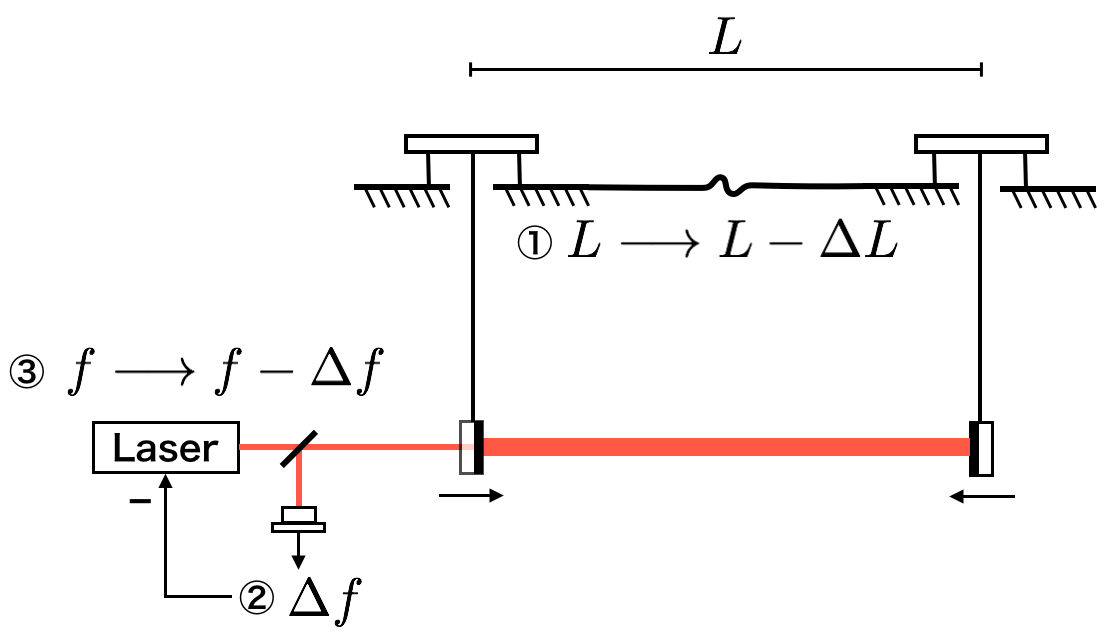
\includegraphics[width=12cm]{./img_chap6/img600.png}
%%     \caption{The designed sensitivity of KAAGRA \cite{akutsu2019first}}{}\label{img:img600}
%%   \end{center}
%% \end{figure}

\subsection{Main Interferometer}
The main interferometer of KAGRA is shown in Figure \ref{img:img601}. The interferometer configuration of KAGRA is also the same as other GW detectors such as advanced LIGO and advanced Virgo, the Michelson interferometer with Fabry-Perot optical cavity on each arm and two recycling optical cavities. The different feature of these detectors is the cryogenic test masses. To cool down to cryogenic, typically 22 K, the test mass mirror is made of sapphire because of the high thermal conductivity and mechanical Q value even in a cryogenic environment. These properties can reduce some problems of the interferometric GW detectors; thermal lens effect and thermal noise.
\begin{figure}[p]
  \begin{minipage}{15cm}
    \begin{center}   
      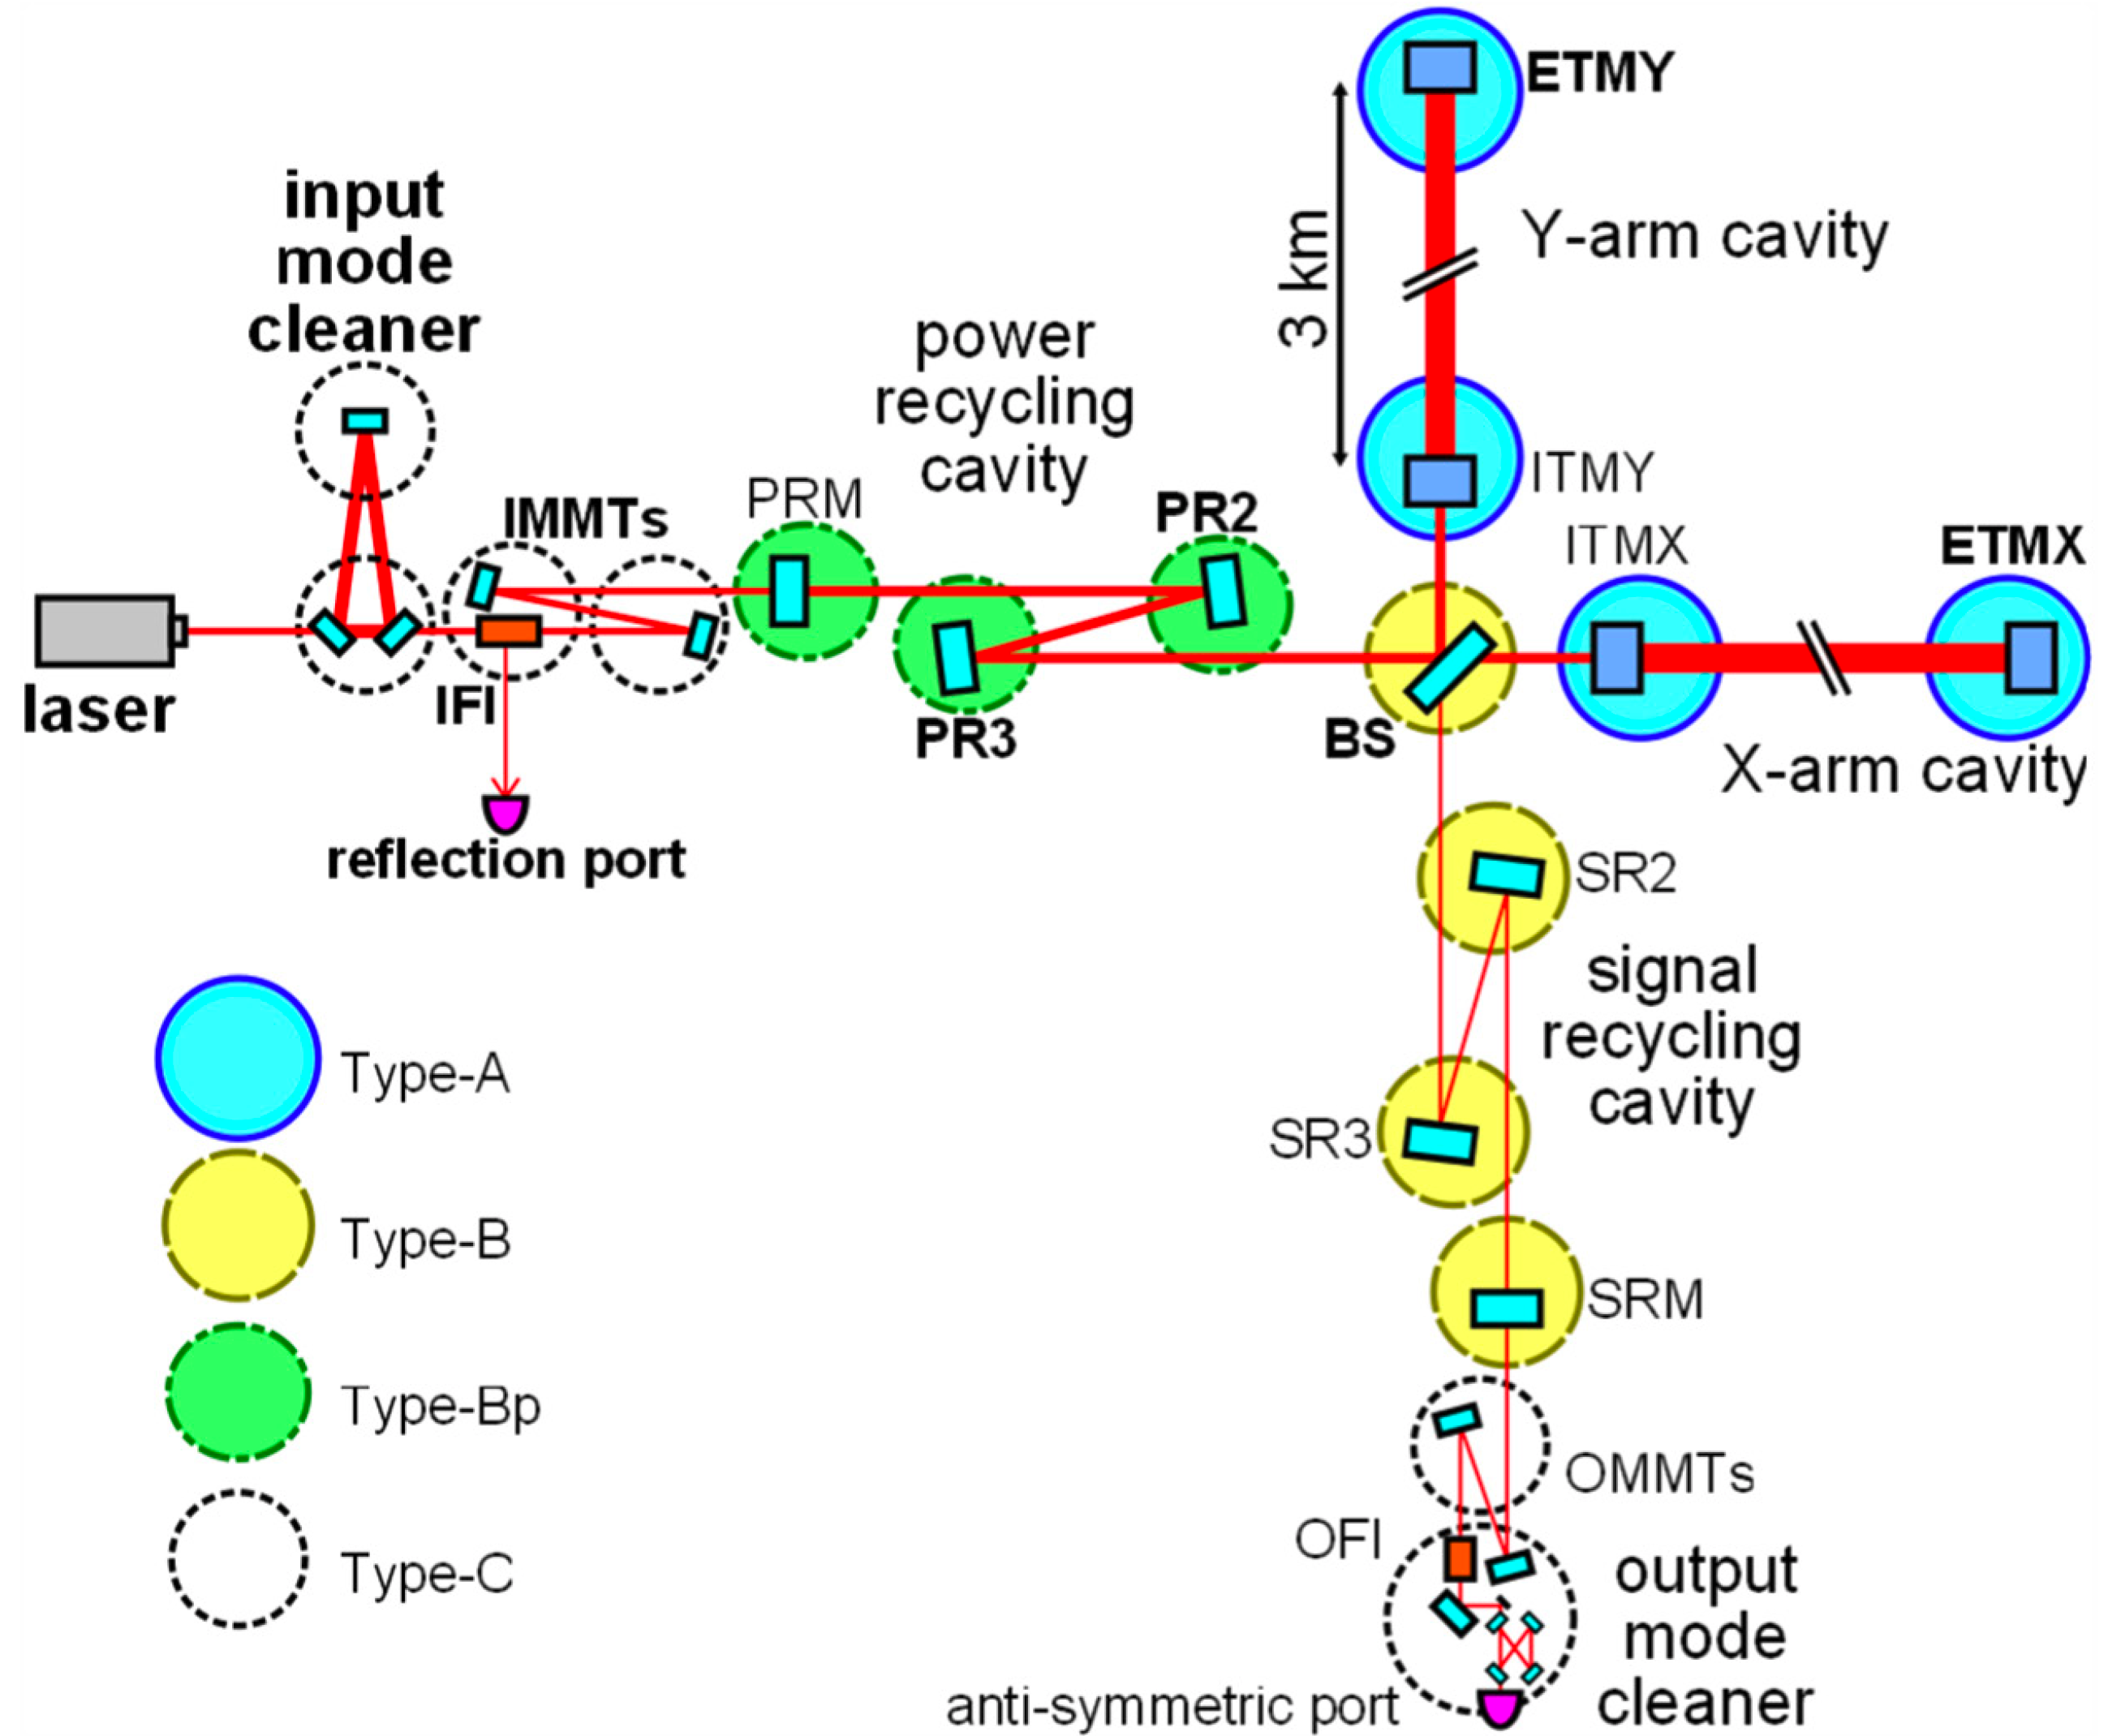
\includegraphics[width=13cm]{./img_chap6/img601.png}
      \subcaption{Schematic interferometer configuration of KAGRA \cite{akutsu2019first}}{}\label{img:img601} \hfill\vspace{10pt}
    \end{center}
  \end{minipage}
  \begin{minipage}{15cm}
    \begin{center}   
      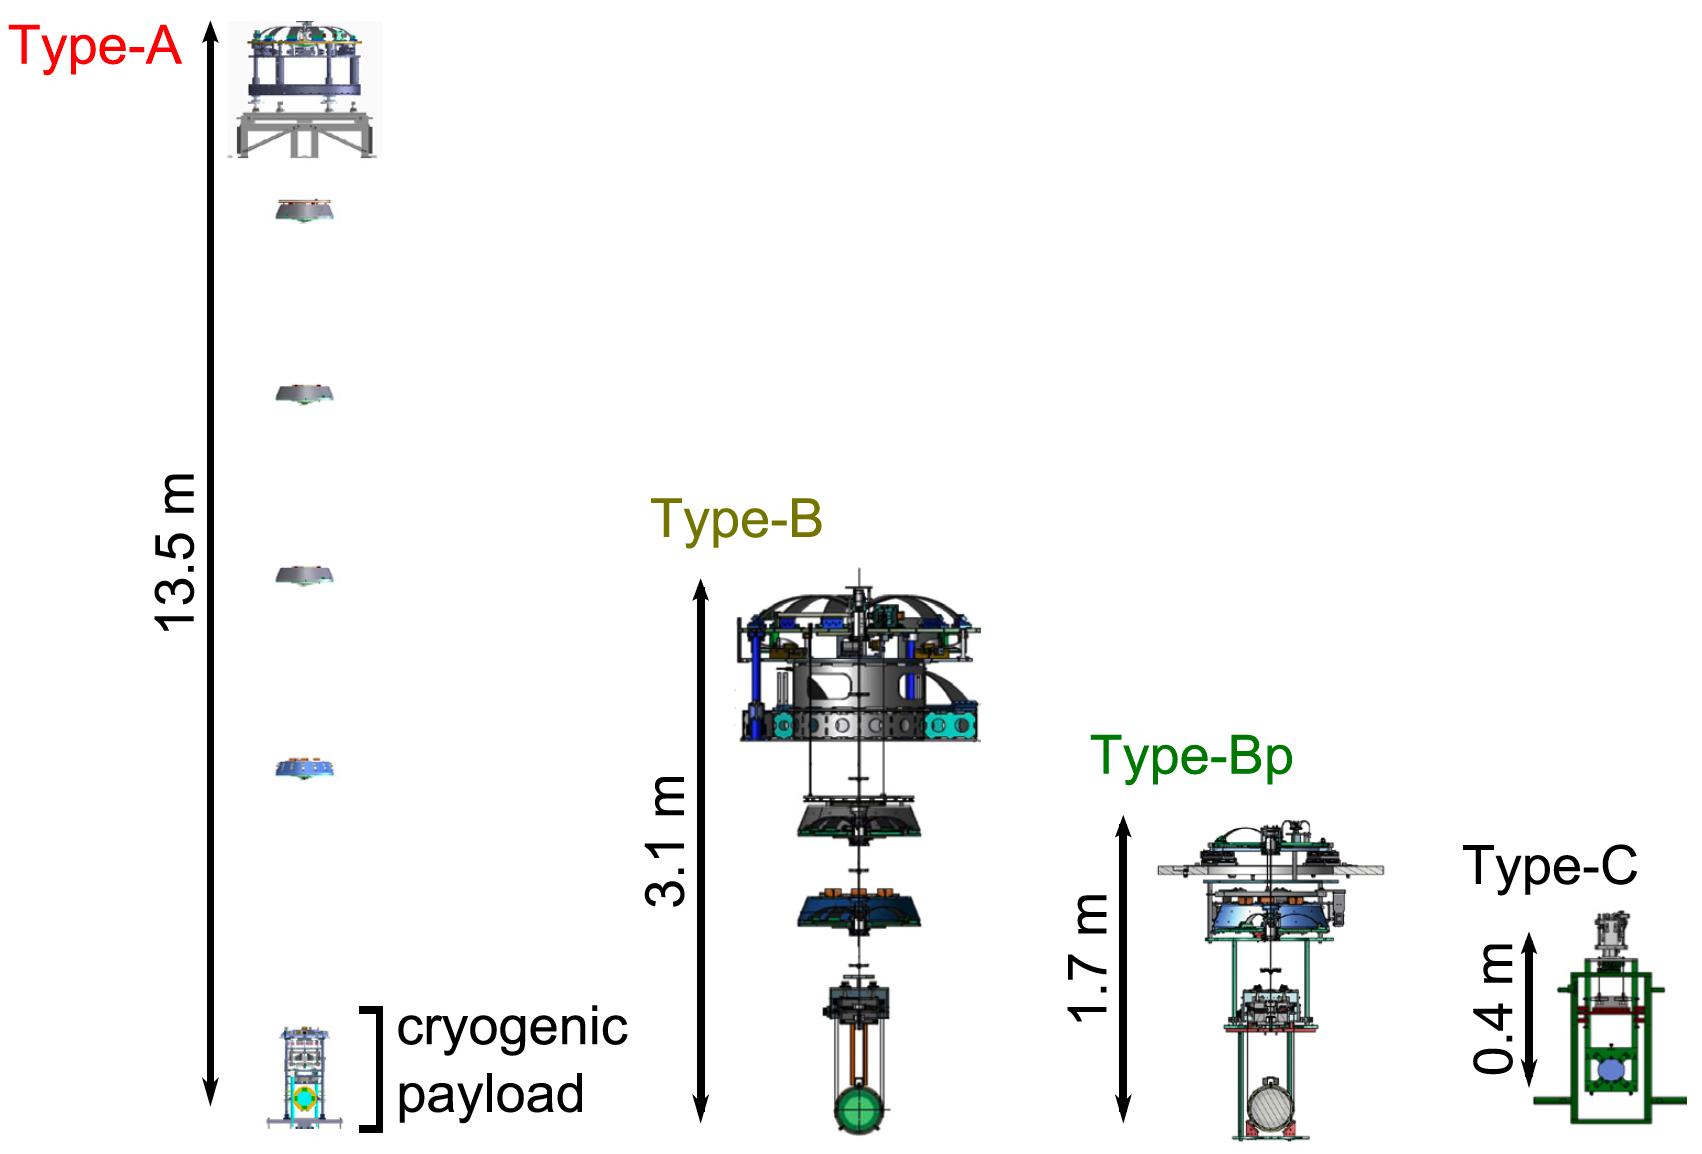
\includegraphics[width=13cm]{./img_chap6/img601b.png}
      \subcaption{KAGRA mirror suspension system \cite{akutsu2019first}}\label{img:img601b}
    \end{center}
  \end{minipage}
  \caption{Interferometer configuration and mirror suspension system}{}
\end{figure}
The main interferometer is divided into four parts; (1) arm cavities, (2) input and output mode cleaners (IMC and OMC), (3) power recycling cavities (PRC), (4) and signal recycling cavities (SRC). The first, the arm cavities are composed of input test masses (ITMs) and end test masses (ETMs) with high reflectivity corresponding to a finesse of 1530 not to increase the internal cavity power. The second, while IMC is used for clean out the higher-order spatial mode and stabilizing the frequency of the main input laser, OMC is used for clean out the unwanted higher-order spatial modes and frequency sideband of the output beam. The IMC is the triangle optical cavity which is made to stabilize the input laser frequency above 1 Hz. The OMC is the bow-tie cavity composed of four mirrors. The third, PRC is used for increasing the input laser power by ten times. This cavity is composed of three mirrors named PRM, PR2, and PR3, respectively. The forth, SRC is used to expand the bandwidth of GW signals. This technique is more important than Advanced LIGO and Advanced Virgo because the bandwidth is narrower than other detectors due to a high finesse arm cavity of KAGRA. 

\subsection{Mirror Suspension System}
All mirrors of the interferometer are suspended by four types of suspensions: Type-A, Type-B, Type-Bp, Type-C. These suspensions are shown in Figure \ref{img:img601b}. The Type-A is a 13.5 m scale 9-stage pendulum suspending the test mass mirror. The Type-B is a small size of Type-A suspension for suspending the signal recycling mirrors and beam splitter mirror. The Type-Bp is also a small size of Type-B but without the pre-isolator stage, which is for the power recycling mirrors. The type-C is the simple 2-stage suspension used in TAMA300 but with minor modification.
\begin{figure}[p]
  \begin{center}   
    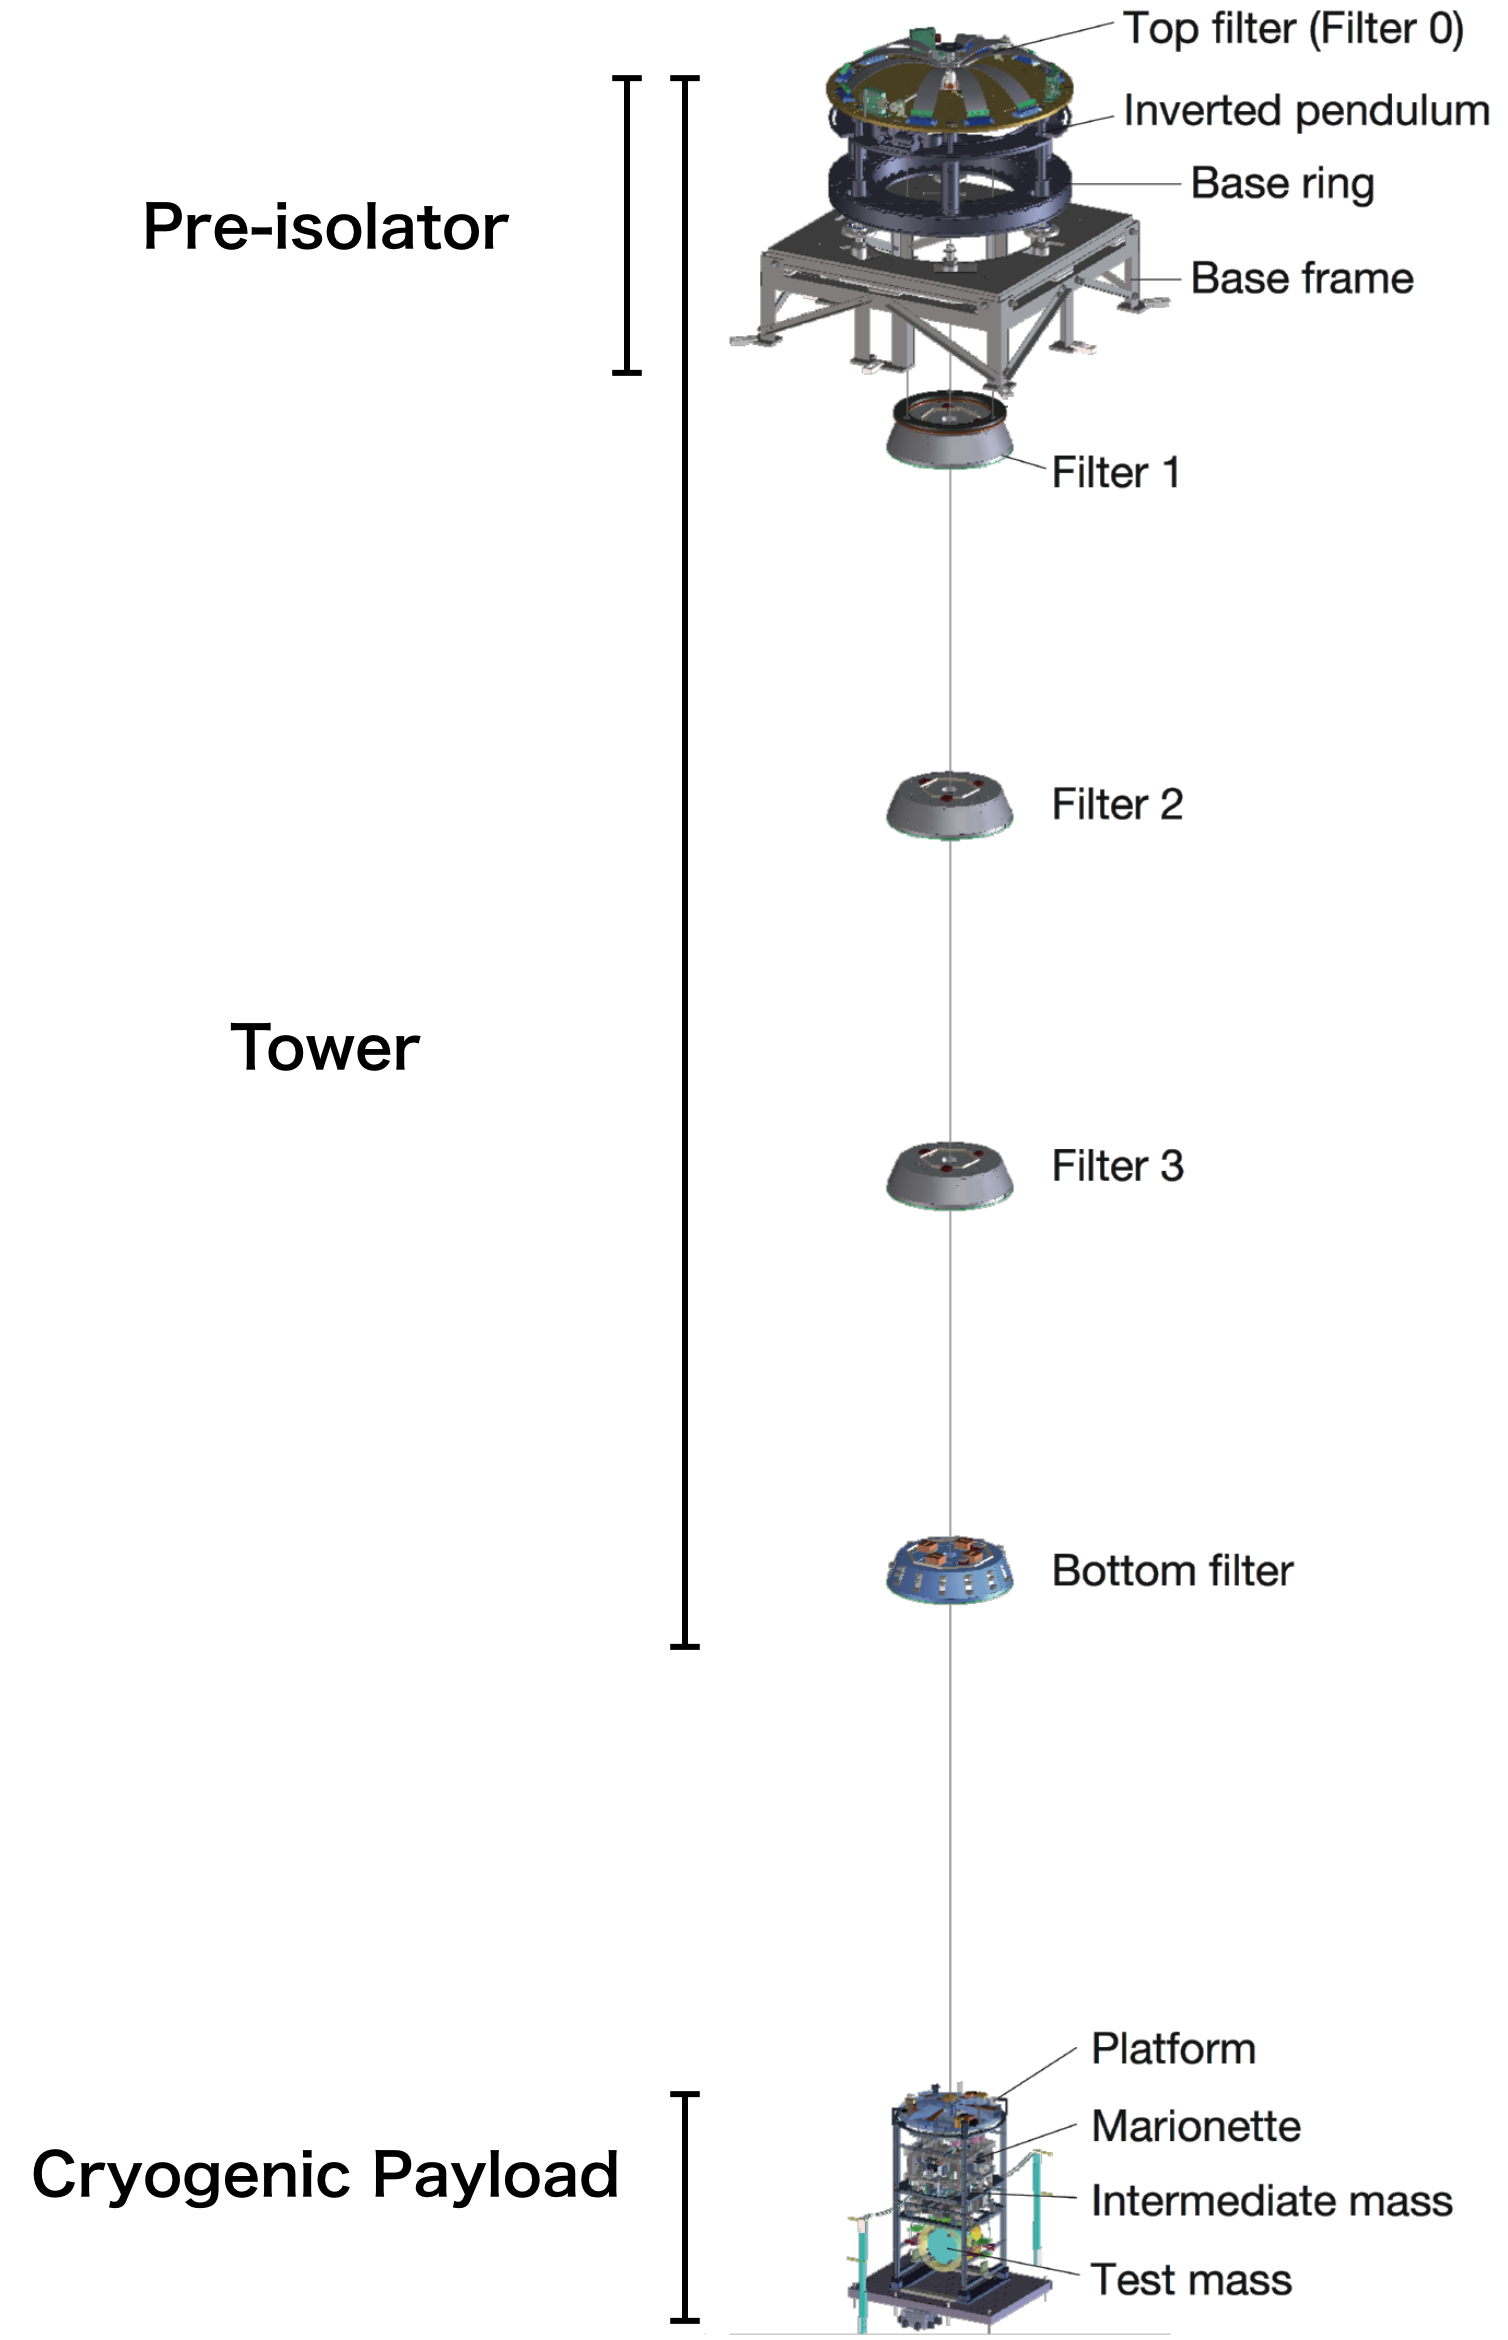
\includegraphics[width=13cm]{./img_chap6/img604.png}
    \caption{An overview of the Type-A suspension \cite{Okutomi2019development}. Test mass is suspended by a $13.5\,\mathrm{m}$ pendulum consisted of several mechanical filters. The suspension point of the long pendulum is supported by the pre-isolator, which consists of an inverted pendulum, on the ground through the base frame and base ring.}\label{img:img604}
  \end{center}
\end{figure}

\begin{figure}[p]
  \begin{minipage}{1.0\hsize}
    \begin{center}   
      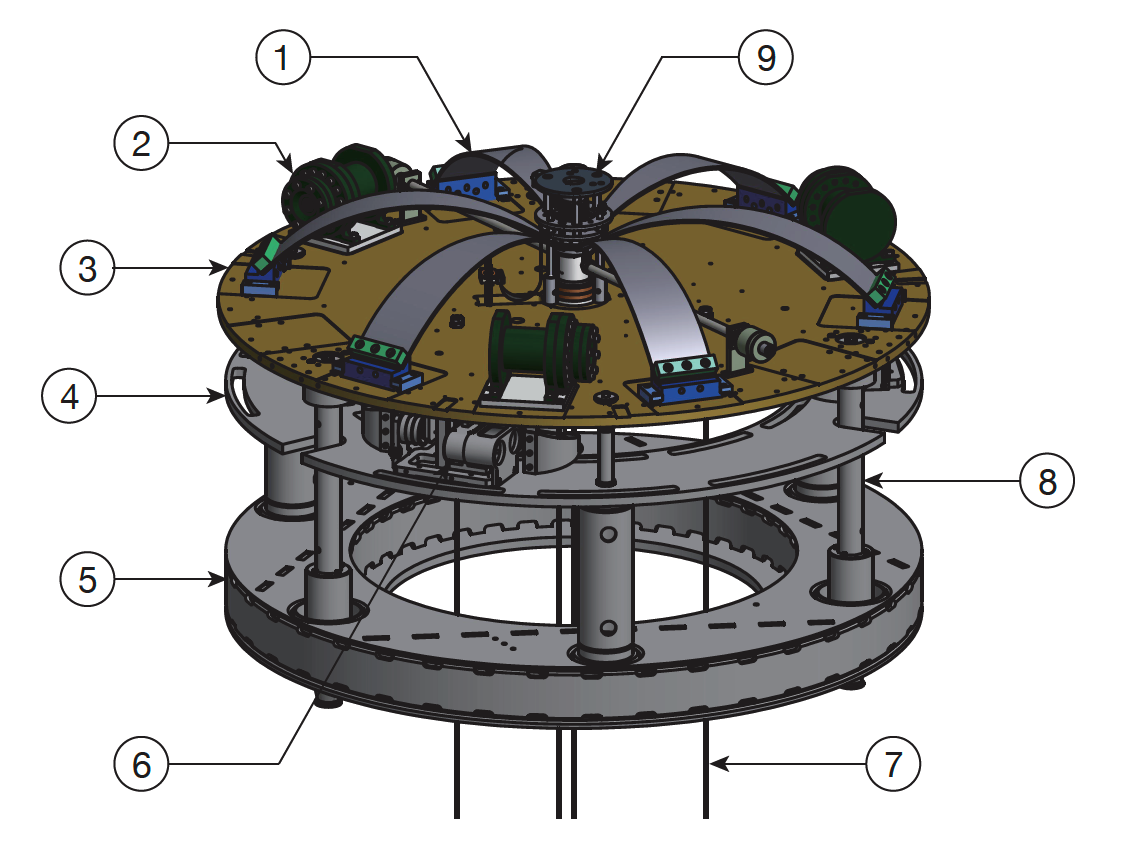
\includegraphics[width=12cm]{./img_chap6/img603a.png}
      \subcaption{Pre-isolator stage (PI). (1) Cantilever blade for GAS. (2) Geophone (3) Table of the top stage (4) Refernce frame rigidly connected to the base ring (5) The base ring mounted on the ground (6) LVDT and the coil magnet actuator (7) suspension wire to suspend the lower stages (8) leg of the inverted pendulum (IP). Figure is cited from figure 3.9 in \cite{Okutomi2019development}}\label{img:img603a}
    \end{center}
  \end{minipage}\\   
  \begin{minipage}[b]{0.5\hsize}
    \begin{center}
      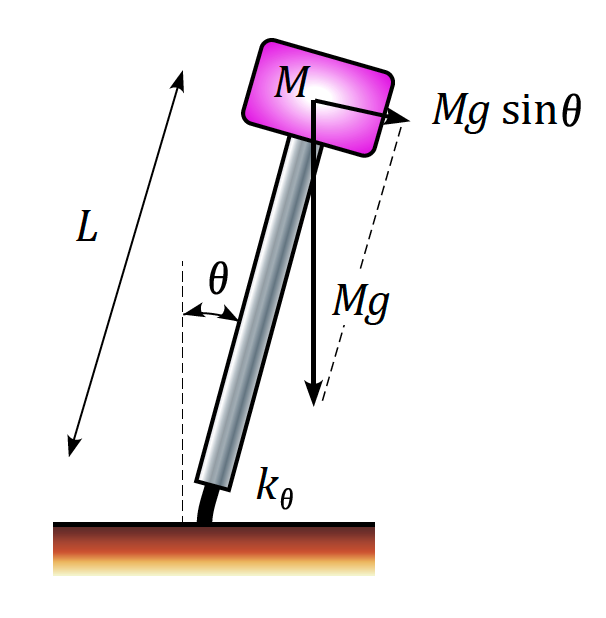
\includegraphics[width=8cm]{./img_chap6/img603b.png}
      \subcaption{Leg of the inverted pendulum (IP) \cite{sekiguchi2016astudy}.}\label{img:img603b}
    \end{center}
  \end{minipage}
  \begin{minipage}[b]{0.5\hsize}
    \begin{center}
      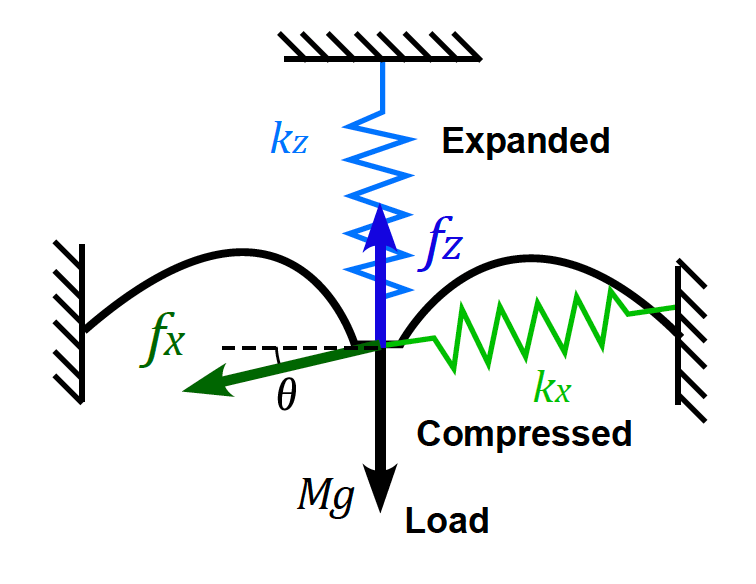
\includegraphics[width=8cm]{./img_chap6/img603c.png}
      \subcaption{Geometrical Anti-Spring \cite{sekiguchi2016astudy}.}\label{img:img603b}
    \end{center}
  \end{minipage}  
  \caption{CAD drawing of the pre-isolator (top) and main mechanical components of PI; IP leg and GAS (bottom).}
\end{figure}


\section{KAGRA Type-A Suspension}
\subsection{Overview}
In order to suspend the cryogenic test mass, as shown in Fig.\ref{img:img604}, KAGRA Type-A suspension has two parts; cryogenic payload and $13.5\,\mathrm{m}$ room temperature tower pendulum \cite{Okutomi2019development}. The cryogenic payload consists of Platform, Marionette, Intermediate mass, Test mass. The tower consists of 5 mechanical filters; Top filter, F1, F2, F3, and Bottom filter. Moreover, the suspension point of the tower is suspended by the pre-isolator stage which has an inverted pendulum.

In terms of the low-frequency seismic attenuation, the pre-isolator is the important mechanical part.



\subsection{Pre-Isolator stage (PI)}
The pre-isolator (PI) is active seismic isolation for the suspension point of the long Type-A or Type-B suspensions. As shown in Figure \ref{img:img603a}, the suspension point is on the platform stage supported by the inverted pendulum (IP) which isolates the seismic noise in a horizontal direction. For vertical direction, geometric anti-spring (GAS) suspends this point. Especially, the horizontal motion of the platform stage is isolated by using the feedback control with the inertial sensor and the relative position sensor.

\subsubsection{Inverted pendulum for horizontal vibration isolation}
Inverted pendulum (IP) is the low eigenfrequency pendulum because this mechanical filter can adjust the effective spring constant to small value by tuning the load on the platform stage. The angular eigenfrequency of the single IP leg is given by \cite{sekiguchi2016astudy}
\begin{eqnarray}
  \omega_{\mathrm{IP}}=\sqrt{\frac{g}{L}\left(\frac{k_{\mathrm{\theta}}/gL-M}{M}\right)},\\
\end{eqnarray}
where $k_{\theta}$ is the bending spring constant of the flexure, $M$ is the mass of the stage, and $L$ is the length of the leg. Although the eigenfrequency can be adjusted to zero in principle, actual eigenfrequency is designed at least 100 mHz because it is unstable when the term in the square root is minus value.

\subsubsection{Geometric Anti-Spring for vertical vibration isolation}
Geometric anti-spring is also the low eigenfrequency pendulum in a vertical direction. The eigenfrequency is adjusted to small value by compressing the cantilever blades as shown in Figure \ref{img:img603b}. The angular eigenfrequency is given by 
\begin{eqnarray}
  \omega_{\mathrm{GAS}} = \sqrt{\frac{1}{M}\left[{ k_{z}- \left(\frac{l_{0}}{x_{0}}-1\right) k_{x}}\right]},
\end{eqnarray}
where $M$ is the load mass, $k_{\mathrm{x}}$ and $k_{\mathrm{z}}$ are the elastic constant of the compressed catilevers, $l_{0}$ is a natural length of the blades, $x_0$ is the horizontal distance between the central keystone and the support poit of the blades. One can find that the angular eigenfrequency of the GAS is reduced when $x_{0}<l_{0}$.

\subsubsection{Liner Variable Differential Transducer (LVDT)}
\begin{figure}[h]
  \begin{center}   
    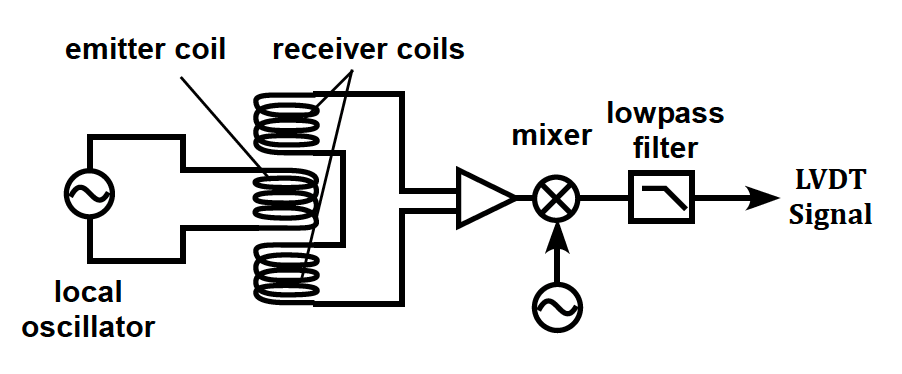
\includegraphics[width=10cm]{./img_chap6/img605.png}
    \caption{\cite{sekiguchi2016astudy}}\label{img:img605}
  \end{center}
\end{figure}
LVDT is a wide range relative position sensor composed of three coils \cite{Tariq2002hh}. shown in Fig.\ref{img:img605}. The emitter coil is mounted on the pre-isolator stage and driven with a sinusoidal signal to emit a modulated magnetic field. The two receiver coils are mounted on the reference structure, and these coils are counter-wound to each other. When the emitter coil is on the center of two receiver coils, the induced voltage is not emitted from the receiver coils. On the other hand, when the pre-isolator is moved, a sinusoidal signal appears on the receiver coils. Therefore, after demodulating this signal, the amplitude of the output signal is proportional to the displacement from the LVDT geometrical center.

\subsubsection{Coil-magnet actuator}
We use a voice-coil type wide range actuator to move the pre-isolator stage \cite{wang2002constant}.


\chapter{Gaussian Beam}
\section{Gaussian beam}
The ideal Gaussian beam has a fundamental spatial mode called $\mathrm{TEM}_{00}$. The whose electric field of the beam propagating to $z$ axis is given by \cite{bond2016interferometer,svelto1998principles}
\begin{eqnarray}
  u(x, y, z)=\sqrt{\frac{2}{\pi{w^2(z)}}} \exp \left(i\zeta(z)-\mathrm{i} k \frac{x^{2} +y^{2}}{2 R(z)}-i\frac{2\pi}{\lambda}z\right)
  \exp \left(-\frac{x^{2}+y^{2}}{w^{2}(z)}\right),  \label{eq:eq415}
\end{eqnarray}
where $\lambda,\,w_0$ are the wavelength and the beam radius at $x=0$ of the beam. In addition,
\begin{eqnarray}
  z_0 &=& \frac{\pi{w^2_0}}{\lambda} \\ \label{eq:eq415_a}
  w(z) &=& w_0\sqrt{1+\left(\frac{z}{z_0}\right)^2}, \\ \label{eq:eq415_b}
  R(z) &=& z\left[1+\left(\frac{z_0}{z}\right)^2\right],\\ \label{eq:eq415_c}
  \phi(z) &=& \arctan\left(\frac{z}{z_0}\right) \label{eq:eq415_d}
\end{eqnarray}
are Rayliegh range and radius, curvature, and Gouy phase of the beam as a function of $z$, respectively. One can find that power of the beam $|u^2|$ has a Gaussian distribution as shown in Figure  \ref{img:img415a} according to Eq.(\ref{eq:eq415}). 

\begin{figure}[p]
  \begin{minipage}{14cm}
    \centering    
    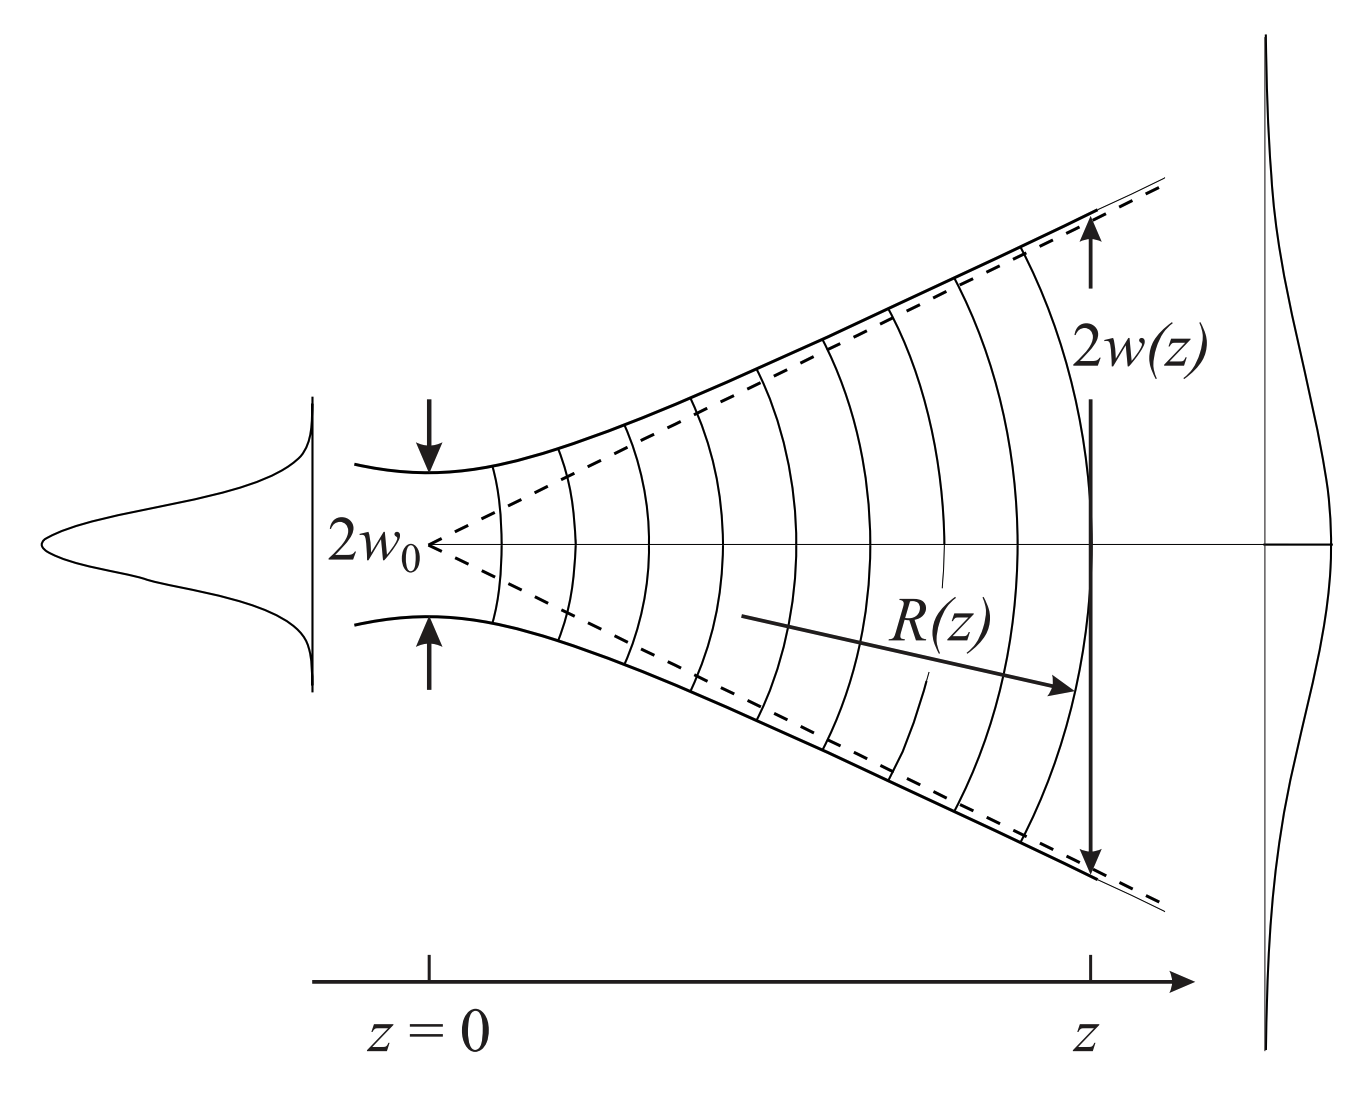
\includegraphics[width=8cm]{./img_chap4/img415a.png}
    \subcaption{Evolution of a Gaussian beam propagating along the z-axis\cite{riehle2006frequency}}{$w_0$ denotes a beam radius at beam weist, where $z=0$. $w(z)$ and $R(z)$ are the beam radius and curvature at $z$. Gouy phase is not shown in here.}\label{img:img415a}
  \end{minipage}\\
  \begin{minipage}{14cm}
    \centering        
    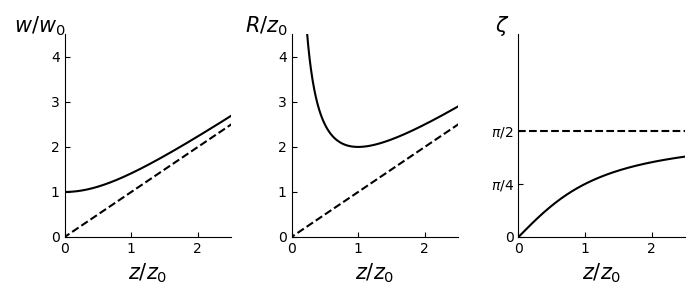
\includegraphics[width=14cm]{./img_chap4/img415.png}
    \subcaption{Beam prifile}{(left) Beam radius normalized by $w_0$ as a function of $z/z_0$, where $z_0$ is Rayleigh length. (Middle) Beam curvature normalized by $z_0$. (right) Gouy phase.}\label{img:img415}    
  \end{minipage}
  \caption{Gaussian beam.}
\end{figure}

As shown in Figure \ref{img:img415}, the beam profiles given by Eq.(\ref{eq:eq415_b},\ref{eq:eq415_c},\ref{eq:eq415_d}) are plotted as a function of $z$. In near-field ($z=0$), the beam can be regarded as the plane wave because the beam radius is smallest (beam waist), and the Gouy phase is 0. On the other hand, in far-field, the beam looks like a point source from far distant, and it is regarded as the spherical wave.
